% -----------------------------------------------
% Template for ICMC SMC 2014
% adapted and corrected from the template for SMC 2013,  which was adapted from that of  SMC 2012, which was adapted from that of SMC 2011
% -----------------------------------------------

\documentclass{article}
\usepackage{icmcsmc2014}
\usepackage[]{biblatex}
\addbibresource{SpatDIF.bib}
\usepackage{times}
\usepackage{ifpdf}
\usepackage[english]{babel}
\usepackage{listings}
\usepackage{enumitem}
\usepackage[export]{adjustbox}
\sloppy

%user defined variables
\def\papertitle{The SpatDIF library -- Concepts and Practical Applications in Audio Software}
\def\firstauthor{Jan C. Schacher}
\def\secondauthor{Chikashi Miyama}
\def\thirdauthor{Trond Lossius}

% pdf-tex settings: detect automatically if run by latex or pdflatex
\newif\ifpdf
\ifx\pdfoutput\relax
\else
   \ifcase\pdfoutput
      \pdffalse
   \else
      \pdftrue
\fi

% \ifpdf % compiling with pdflatex
  \usepackage[pdftex,
    pdftitle={\papertitle},
    pdfauthor={\firstauthor, \secondauthor, \thirdauthor},
    bookmarksnumbered, % use section numbers with bookmarks
    pdfstartview=XYZ % start with zoom=100% instead of full screen; 
                     % especially useful if working with a big screen :-)
   ]{hyperref}
  \pdfcompresslevel=9

  % \usepackage[pdftex]{graphicx}
  \usepackage{graphicx}
  \usepackage[export]{adjustbox}
  \DeclareGraphicsExtensions{.pdf,.jpeg,.png}

  \usepackage[figure,table]{hypcap}
	
% \else % compiling with latex
%   \usepackage[dvips,
%     bookmarksnumbered, % use section numbers with bookmarks
%     pdfstartview=XYZ % start with zoom=100% instead of full screen
%   ]{hyperref}  % hyperrefs are active in the pdf file after conversion
% 
%   \usepackage[dvips]{epsfig,graphicx}
%   % declare the path(s) where your graphic files are and their extensions so 
%   %you won't have to specify these with every instance of \includegraphics
%   \graphicspath{./figures/}
%   % \DeclareGraphicsExtensions{.eps}
% 
%   \usepackage[figure,table]{hypcap}
% \fi

%setup the hyperref package - make the links black without a surrounding frame
\hypersetup{
    colorlinks,%
    citecolor=black,%
    filecolor=black,%
    linkcolor=black,%
    urlcolor=black
}
\hyphenation{SpatDIF} % prevents potential linebreaks within SpatDIF
\usepackage{color}
\definecolor{carrotorange}{rgb}{0.93, 0.57, 0.13}
% \newcommand{\np}[1]{\noindent\textcolor{carrotorange}{[\underline{NP:} #1]}}
\newcommand{\todo}[1]{\noindent\textcolor{red}{[\underline{TODO:} #1]}}
\title{\papertitle}

% Authors
% Please note that submissions are NOT anonymous, therefore 
% authors' names have to be VISIBLE in your manuscript. 

 \threeauthors
   {\firstauthor} {Zurich University of the Arts\\
   Institute for Computer Music\\ and Sound Technology ICST\\
     {\tt \href{jan.schacher@zhdk.ch}{jan.schacher@zhdk.ch}}}
   {\secondauthor} {University of Music, Cologne\\ 
   Studio for Electronic Music\\
     {\tt \href{me@chikashi.net}{me@chikashi.net}}}
   {\thirdauthor} { Bergen Center for Electronic Arts BEK\\ %
     {\tt \href{trond.lossius@bek.no}{trond.lossius@bek.no} }
}

\begin{document}

\capstartfalse
\maketitle
\capstarttrue

\begin{abstract}
The development of SpatDIF, the Spatial Sound Description Interchange Format, continues with the implementation of concrete software tools.
In order to make SpatDIF usable in audio workflows, two types of code implementations are developed.
The first is the C/C++ software library `libspatdif', whose purpose is to provide a reference implementation of SpatDIF.
The class structure of this library and its main components embodies the principles derived from the concepts and specification of SpatDIF.
The second type of tool are specific implementations in audio programming environments, which demonstrate the methods and best-use practices for working with SpatDIF.
Two practical scenarios demonstrates the use of an external in MaxMSP and Pure Data as well as the implementation of the same example in C++.
A short-term goal is the complete implementation of the existing specification within the library. 
A long-term perspective is to develop additional extensions that will further increase the utility of the SpatDIF format.

\end{abstract}

% keywords: spatial sound, scene description, software implementations, best-practice

\section{Background}\label{sec:background}

The Spatial Sound Description Interchange Format (SpatDIF) presents a structured syntax for describing spatial audio information, addressing the different tasks involved in creating and performing spatial sound scenes.
The goal of this approach is to simplify and enhance the methods of creating spatial sound content and to enable the exchange of scene desriptions between otherwise incompatible software. 
SpatDIF proposes a simple and extensible format as well as best-practice examples for storing and transmitting spatial sound scenes. 
It encourages portability and the exchange of compositions between venues with different surround audio infrastructures. 
SpatDIF also fosters collaboration between artists such as composers, musicians, sound installation artists as well as researchers in the fields of acoustics, musicology, and sound engineering.
SpatDIF was developed in a collaborative effort and has evolved over a number of years.
% \subsection{Project History}\label{subsec:project_history}
% COMMENT: Do we need to recap all of the history of SpatDIF? Isn't this already covered in the CMJ paper? If we save some space here, we could make figure 1 larger.
%SpatDIF was coined in \citeyear{peters_caa07} \cite{peters_caa07} when Peters~et.~al. posited the need for a format describing spatial sound scenes in a structured way, since at that time all of the available spatial rendering systems used self-contained, proprietary syntax- and data-formats.
%Through a panel discussion \cite{2008ICMCpanel, Peters:2008spatdif} and other meetings and workshops, the scope and concepts of SpatDIF were extended, refined, and consolidated.
%After an extended process the SpatDIF specification was informally presented to the spatial sound community at the ICMC in Huddersfield in August 2011 and at a workshop at the TU-Berlin in September 2011.
%The responses in these meetings suggested the urgent need for a lightweight and easy to implement spatial sound scene standard, which would contrast the complex MPEG-4 scene description specification \cite{scheirer1999audiobifs}.
The completion of a first usable version of the specification \cite{SpatDIF_03} defining the core descriptors and a few indispensable additional descriptors was achieved in 2012 and is published in the Computer Music Journal \cite{Peters:2013SpatDifCMJ}.
The community pages as well as all the related information can be found at \href{http://www.spatdif.org}{www.spatdif.org}.\footnote{All URIs in this article were last accessed in April 2014.}

Since SpatDIF is a syntax rather than a programming interface or file-format it may be represented in any of the current or future structured mark-up languages or messaging systems.
It describes only those aspects required for the storage and transmission of \emph{spatial scene descriptions}.
Because a complete work typically contains aspects that are outside the realm of spatial sound scenes, SpatDIF provides descriptors to link these aspects to the spatial dimensions, but only to the extent necessary.
% \subsection{Design Principles}\label{subsec:design_principles}
% We have now started to implement the concepts in actual software.

A central principle for SpatDIF is the separation of authoring and rendering of spatial sound scenes or pieces.
They may occur at separate times using the same or differing infrastructure, at separate places either simultaneously or with a long time between the two, and through a mixture of these factors. 
The exact modality should not have to be determined at the outset.
In addition to the separation of the basic functionalities two principal use-cases can be distinguished.
The first scenario is focusing on storing spatial audio scene descriptions for future playback. 
The second scenario deals with streamed audio content and scene description information in real- and near real-time.
For these applications SpatDIF formulates a concise semantic structure that is capable of carrying all the information relevant for preserving a sound scene, without being tied to a specific implementation or technical method.
% For example, the description of media-streams in SpatDIF is necessary in order to define the storage location or origin of the audio present in the scene.
% For example, to be able to render the audio objects with the correct audio content in the spatial scene, the storage location of the audio content needs to be defined via SpatDIF's media resources.
For example, the description of media-streams in the Media extension is necessary in order to describe from where the sounding content of the scene originates.

\section{Library Concepts}\label{sec:libspatdif_concepts}

% COMMENT: The structure of the two paragraphs in this section could be improved. Would it be better to have a first paragraph on the lib, and a second on the implementations?
After establishing a coherent specification with example use-cases in textual form only, the next development step is the implementation of software, which embodies the specified concepts and should serve as a reference for future work.

In this article we present the development and implementation of software tools aimed at easy integration of SpatDIF into existing software and workflows.
The concepts and guidelines laid down in the SpatDIF specification are implemented in a platform-independent software library written in C/C++ \cite{Miyama_2013}.
The library is in charge of holding one or more spatial audio scenes and provides ways to read and write elements to and from this scenes, either directly from native code or via OSC-formatted messages, that may originate from within the application or arrive from an external source via the network.
By providing a software library rather than just a complete software application, implementations in many different software environments are facilitated, which is one of the goals of the project.

In section \ref{sec:examples} the application of the library will be demonstrated in an external for MaxMSP\footnote{\href{http://www.cycling74.com}{www.cycling74.com}} and PureData \footnote{\href{http://puredata.info}{puredata.info}} as well as in an application written entirely in C++ in OpenFrameworks.\footnote{\href{http://www.openframeworks.cc}{www.openframeworks.cc}}

\subsection{Scope of Library Tasks}\label{subsec:separation}

In order to facilitate implementations in many different environments without making any assumptions about their capabilities, the types of tasks given to the library is carefully selected.
There is a deliberate division of tasks between the library and the client application.

On the one hand, the library builds and maintains in memory the SpatDIF scene, either obtained from an already existing description stored in a file, or on-the-fly in real time from elements received via OSC-formatted commands or native code calls.
It provides an application programming interface (API) that hides most of the complexity of handling the scene data.
Through this interface all the information is queried or written.

The client application, on the other hand, is in charge of connecting to the file-system, managing the networking interfaces as well as running the audio-system.
All time-based operations are done in the client-application, since they may be driven by audio-rate, a control-rate scheduler or even an external sync source. 
The client application deals with all audio-related processes, such as loading audio files, playing them back, configuring the audio-system and rendering the audio to generate an immersive audio experience.
% More details of how the tasks are divided are shown below in the sections describing the specific examples.


\begin{figure}[bh]
	\centering
	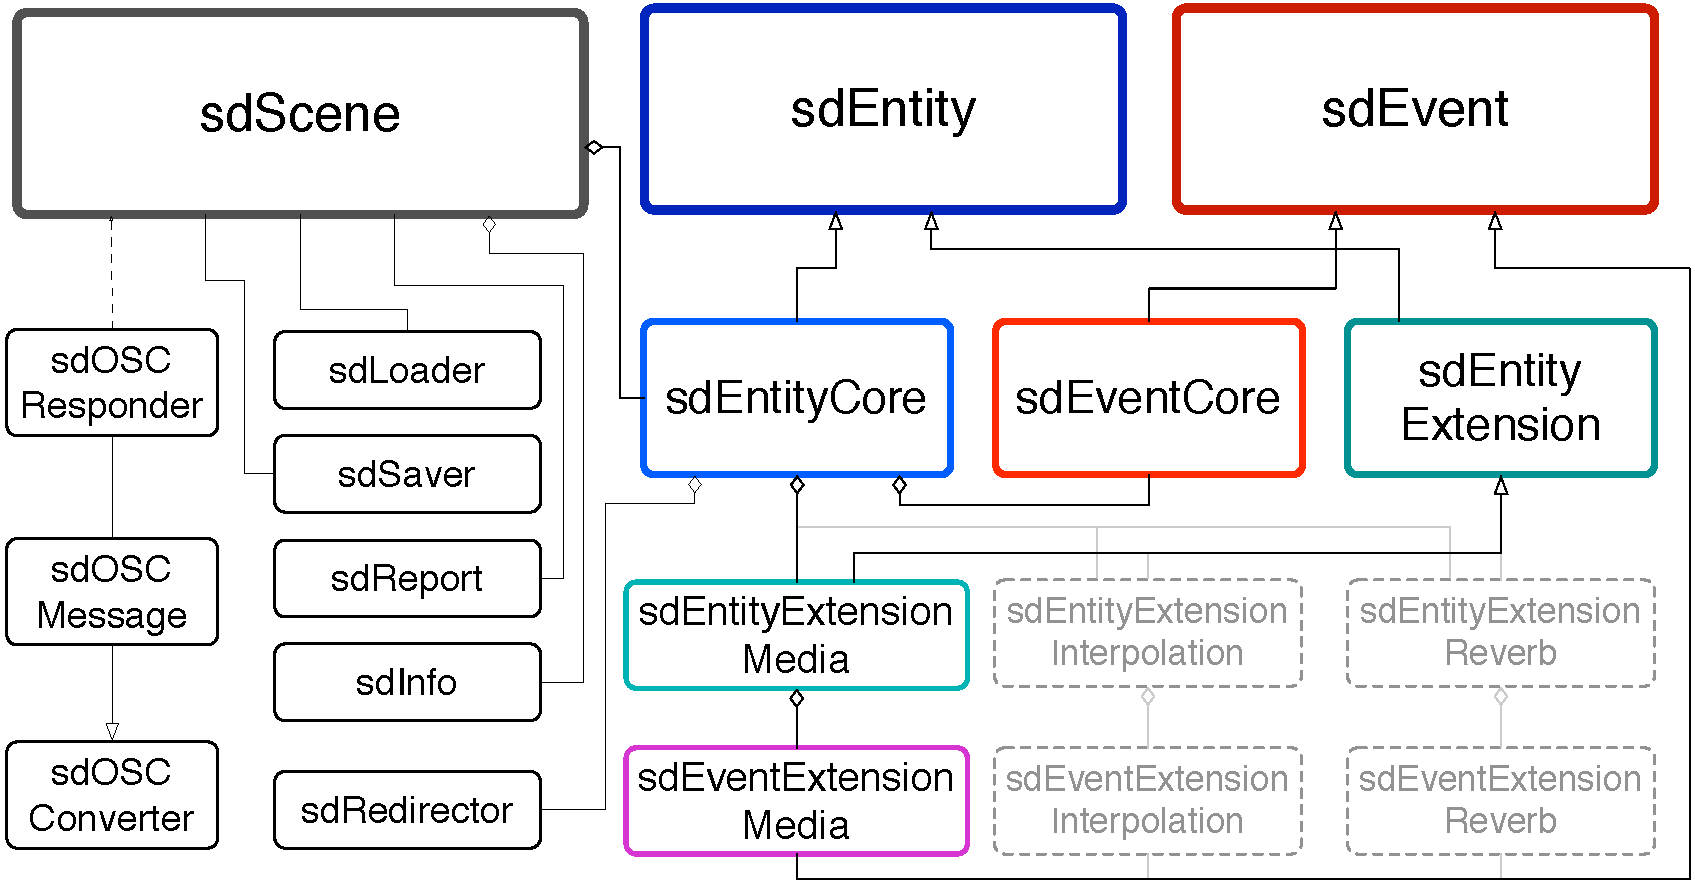
\includegraphics[width=\columnwidth]{class_diagram.pdf}
	\caption{Simplified class hierarchy of the SpatDIF software library. The top row shows the three main classes, below are their derived subclasses. Interfacing and utility classes are placed on the left and future extensions on the right are marked in dashed grey.}
	\label{fig:class_structure}
\end{figure}

\subsection{Library Class Structure}\label{subsec:class_structure}

The class diagram in Figure \ref{fig:class_structure} illustrates the relationship between the scene and its contents, as well as their hierarchical dependencies.
An instance of \emph{sdScene} class represents a SpatDIF scene and maintains instances of \emph{sdEntityCore}.
Core classes cover the elements mandated by SpatDF while extension classes introduce additional and optional descriptions.
The functionalities of \emph{sdEntityCore} may thus be extended by the descendants of \emph{sdEntityExtension}. 
The activation and deactivation of the extensions is managed globally within a scene, therefore \emph{sdScene} is responsible for all extension handling.
Each instance of \emph{sdEntityCore} maintains instances of \emph{sdEvent}, which represent all the events of the entity as they unfold within the scene over time.

The following are brief descriptions of the most important classes.


\subsubsection*{sdScene}
An instance of \emph{sdScene} maintains all data associated to a SpatDIF scene.
This class offers clients the addition, deletion and modification of \emph{entities} in the scene, the addition and modification of the \emph{meta data} associated with the scene, and finally the activation and deactivation of \emph{extensions} in the scene.

Once the client activates an extension in a scene, \emph{sdScene} automatically adds extended functionalities and allocates extra buffers to all existing and newly created instances of \emph{sdEntityCore}. 
Symmetrically, when deactivating an extension, \emph{sdScene} removes all extended functionalities and previously allocated buffers from all existing \emph{sdEntitieCores}, leading to the deletion of all data stored in the extension buffers.

\subsubsection*{sdEvent}
This is a pure abstract class holding events, storing the absolute \emph{time} of the event, a \emph{descriptor} of the type of event, and the actual data as a \emph{value}.

\subsubsection*{sdEntity}
This class defines entities in SpatDIF scenes as a pure abstract class. It implements basic functionalities, such as addition, deletion, and modification of events.

\subsubsection*{sdEntityCore}
An instance of \emph{sdEntityCore} maintains events with SpatDIF core descriptors and a vector storing instances of SpatDIF extensions. 
This class replies to queries from the client about events, e.g., if a client asks an \emph{sdEntityCore} for a value of a certain descriptor at a specific time. 
The client is able to query about multiple events within a certain time frame and filter events by descriptors. 

\subsubsection*{sdEntityExtension}
This is a pure abstract class of extensions, and the descendants of this class. e.g., \emph{sdEntityExtensionMedia}, handle the events with extended descriptors. 
If a client activates an extension in a scene, each existing instance of \emph{sdEntityCore} instantiates the designated subclass of \emph{sdEntityExtension} and registers it.

\subsubsection*{sdLoader/sdSaver}
These two classes provide several utility functions and enable clients to create or store an instance of \emph{sdScene} to/from a XML, JSON, or YAML string. 
In order to maintain platform independence and to achieve maximum flexibility, the library does not handle files directly, the client software is responsible for the file management. 
These functions use two external libraries for parsing of markup formatted strings: TinyXML-2\footnote{\href{http://www.grinninglizard.com/tinyxml}{www.grinninglizard.com/tinyxml} } and libjson\footnote{\href{http://sourceforge.net/projects/libjson}{sourceforge.net/projects/libjson} }.

\section{Practical Implementations}\label{practical_usage}

The SpatDIF syntax is an implementation-independent specification, rather than a specific software interface. 
However, the actual value of using it only becomes evident in real applications. 
Although SpatDIF was developed with a number of different scenarios in mind, the use-case most closely associated with the authors' practices are electro-acoustic surround audio compositions for concerts and installations or real-time spatialisation in computer music performance.
Therefore, the first code implementations of the SpatDIF library are made with tools for real-time audio software.

In order to explore the methods and actual handling of the `libspatdif' in a real situation, a dual testbed was implemented as an external for both MaxMSP and Pure Data, named `spatdif'.
Apart from small differences in the two environments, mainly concerning the handling of files, the two implementations are identical.
In addition, an example application with a limited feature-set was written in openFrameworks, in order to establish and test a workflow done entirely in the C++ language.

There are a number of concepts that need to be taken into account when using the library, informing the design of the implementations shown here.
The library serves as a data-storage for audio scenes that needs to be queried for its information in specific ways.
It does not provide a scheduling mechanism of its own, rather, the client application is responsible for executing all time-related functions.
This design choice is explicitly geared towards temporal flexibility, e.g., slowing down or speeding up playback, jumping and cueing, which are features that can only properly be implemented by the client application.

There are two main interfaces for the library, the native command and the OSC-command, as will be discussed in section \ref{subsec:recording}.
The native commands call functions of the library within C/C++ code whereas the OSC-commands get handed to the library as messages conforming to the OSC syntax.
The library does not implement network socket handling functionalities itself, this is the responsibility of the client environment.
In order to input and output information directly to and from the scene, the name-space is described with hierarchical addresses that must conform to the SpatDIF specification.
In the implementation of the external, the input of elements into the scene adhere to the OSC-style with a slash delimited format, whereas for the outputs from the external, the addresses are converted to a space-delimited format in order to avoid the dependency on an additional OSC-parser.

Additional commands that directly address functions of the library have a different syntax, which is not part of the SpatDIF specification, but instead are specific to the implementation of the library.
These \emph{/spatdifcmd} messages concern the querying of information from the library and the setting and getting of variables necessary for the executing the queries.

File operations are not functions of the library itself.
The external in MaxMSP and PureData implements the required file loading and saving methods, which are specific to their own environment. 
  
\subsection{Example Scene}\label{sec:examples}

For the following examples we use the canonical piece `Turenas' by John Chowning \cite{chowningturenas} (see also \cite{Peters:2013SpatDifCMJ}) , 
The beginning of the SpatDIF scene, including only the `insect' trajectory at second 0:44, contains the following elements in an XML file format:

\lstinputlisting[tabsize=3,columns=fullflexible,breaklines=true,numbers=none,language=XML,morekeywords={source,sink,time,meta},basicstyle=\scriptsize\ttfamily]{turenas_insect_example.xml} 

The corresponding sound files have to be stored and transported alongside to the SpatDIF file.
It is therefore important to think in terms of ‘SpatDIF bundles’ or projects rather than single files. 
We deliberately choose not to propose a container that combines sound files and scene descriptors in a binary format, since human-readability without additional software tools would have been lost. 
 
\begin{figure}[httb]
	\centering
	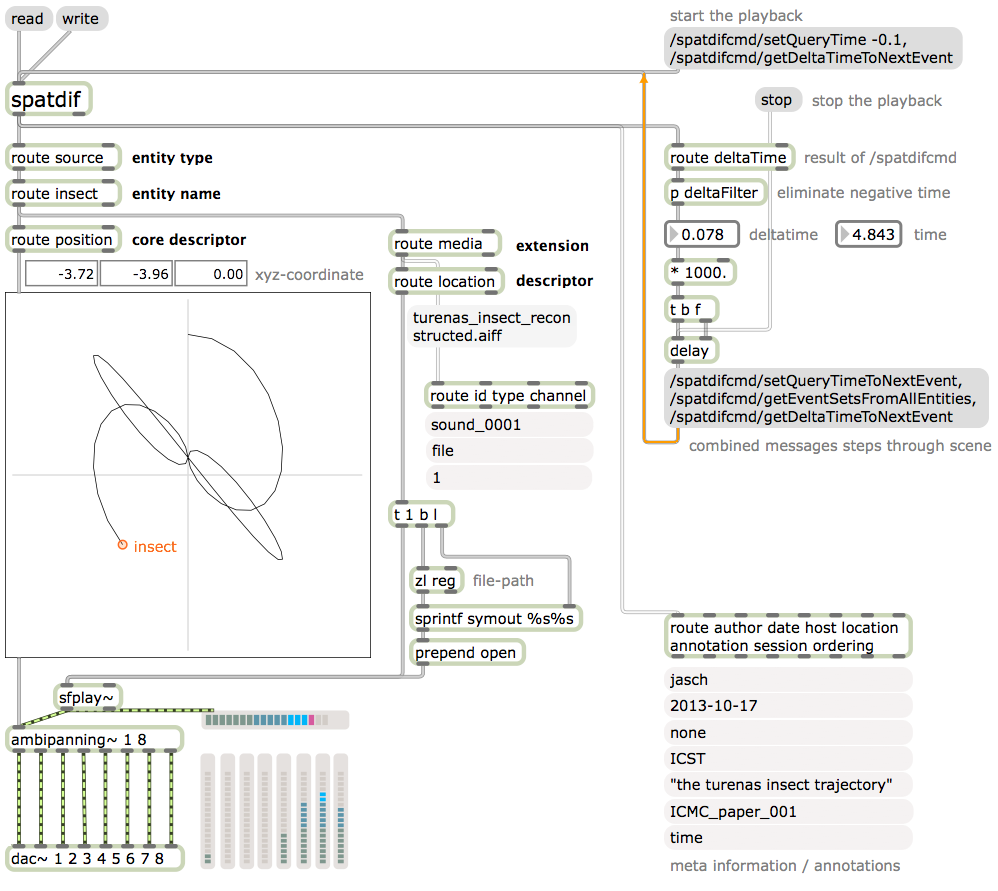
\includegraphics[width=\columnwidth]{playback_maxpatch.png}
	\caption{Implementation of SpatDIF in a MaxMSP external, demonstrating the playback of the Lissajous trajectory from Chowning's `Turenas'.} 
	\label{fig:screenshot}
\end{figure}

\subsection{Playback}\label{subsec:playback}

The first example shown here centres around file-handling and the playback of a SpatDIF scene in a multichannel setup.
Figure \ref{fig:screenshot} shows this with a simplified monophonic setup in MaxMSP.
This workflow makes a few assumptions which are not limitations of libspatdif as such, but reductions that help to clarify the concepts.
The program demonstrates the rendering of the above scene.
The scene is stored on disk in a SpatDIF-formatted XML-file together with the audio content as a sound file.
After reading the scene from disk, the meta section can be parsed in order to obtain annotation information, as shown in the lower right.

In a fully dynamic system, additional information is required to set up the rendering algorithm.
For this purpose queries are made to the library to obtain information about the number of entities present in the scene and the names of the entities as well as the extensions that are present.\footnote{For more specific information about the concept of extensions in SpatDIF, please refer to \cite{SpatDIF_SMC12, Peters:2013SpatDifCMJ, SpatDIF_03}. }
This allows to determine the number of playback voices needed, so that hierarchical message routing can be set up according to the names of entities.
In the example this step is omitted and only one playback voice is implemented with a hard-coded message-routing set to the entity-type of \emph{source} and the entity-name called \emph{insect}.
Subsequently, the messages are routed to obtain the \emph{position} core-descriptor required for the spatialisation process as well as the \emph{media} extension with the \emph{location} descriptor necessary to load files for playback.
The sound file player, visualisation and spatialisation algorithms \cite{Schacher_ICMC_2006} shown here represent the minimal case and would normally be more fully implemented. %\cite{schacher7Years}

As mentioned earlier, the scheduling of events in time is a task of the client application. 
In this example that functionality becomes necessary and therefore a method for time-based playback is demonstrated.
The \emph{spatdifcmds} necessary to run iteratively through the scene can be seen in the right half of the example patch.
The basic action is to ask with \emph{getDeltaTimeToNextEvent} for the delta times between subsequent events.
Since a scene can contain sparse data at no fixed intervals, it is crucial to have a dynamic timing mechanism for playback.
The command \emph{setQueryTimeToNextEvent} sets the query time variable to the next event, then the library gets queried for all the events at that point in time with \emph{getEventSetsFromAllEntities}, and finally the time to wait until the next event is queried again.
These commands form a loop that steps through the scene, which is rendered visible in the figure through the orange connection flowing back to the spatdif external.
The timing is executed by a delay which waits the appropriate amount of time to the next event before re-triggering the same sequence.
These commands are global to the scene, so that all events associated with any entity in the scene are retrieved.
If only events from selected entities are desired, this can be achieved by filtering in the message routing system, or as will be shown below with more specific commands to the library. %TODO find out if we we provide other interface calls to the library across the OSC-cmd interface.

\subsection{Recording}\label{subsec:recording}

In the second example shown in Figure \ref{fig:screenshot2}, spatialisation information originating from real-time input via a physical controller is recorded into a SpatDIF scene.
Four joysticks are set up to control the playback and spatialisation of four monophonic point-source entities in a scene.
As in the previous case, this example is a simplification of a real application, yet still represents a fully functional implementation.
The patch is divided into two processes that run in parallel, the recording on the right side depending on the
realtime processing on the left.
 
In the left half of the Figure \ref{fig:screenshot2}, the real-time process starts from the controller-input and leads to sound spatialisation and multichannel output.
The controller-input at the top feeds into a visualisation-tool before reaching directly the spatialisation-module.
Underneath, keyboard-commanded start/stop switches and file-selection menus control four sound file playback modules.

On the right hand side of Figure \ref{fig:screenshot2} are the parts necessary to record the key-events into a SpatDIF-scene.
The large message-box in the right shows the initialisations necessary to set up the scene.

In this example, each voice independently activates the recording of position information in synchrony with its file-playback.
This mechanism is shown in the `p voice' sub-window. 
Here, the \emph{setPosition} spatdif command is formatted with the correct entity-name and combined with the real-time position data arriving from the visualisation tool.
Further spatdif commands to set media events are \emph{/media/setType} and \emph{/media/setLocation}.
They are tied to specific entities, and therefore need to be formatted with the entity-name and combined with the file-type and file-path of the media resources.

\begin{figure}[httb]
	\centering
	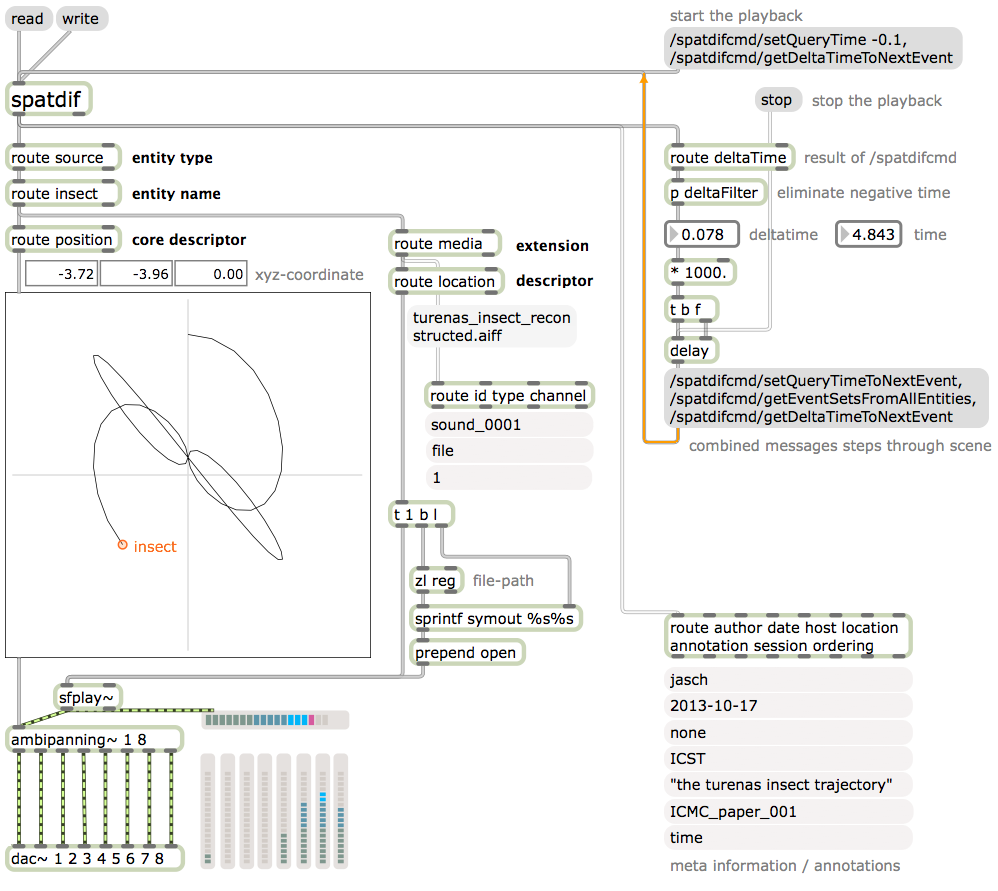
\includegraphics[width=\columnwidth]{recording_maxpatch.png}
	\caption{MaxMSP implementation, demonstrating the recording of four manually generated trajectories obtained from joysticks. The upper right shows the `voice' section responsible for formatting the media and position inputs.} 
	\label{fig:screenshot2}
\end{figure}

Once the media- and position-commands are formatted, they are sent directly to the spatdif external for storage with a time-stamp obtained from the system.
This time-stamp is calculated as relative time since the beginning of the recording and is represented in seconds, formatted as doubles, i.e. 64-bit floating point values.
% COMMENT: Here we have a potential problem: With 32-bit applications (such as Max 32-bit and Pd) we will be unable to preserve 1 ms precision after approx 16:40 minutes... (which, according to some, is the standard length of tape-piece in electro-acoustic music anyways ;=)

The \emph{setWriteTime} commands sets the writing `cursor' in the scene, which will apply to all messages that arrive until a new value for the `writeTime' variable is set.
Grouping all incoming events in this way may be regarded as a type of `frame-based' time-stamping and is defined in the SpatDIF-specification as a scene ordered according to time.

A `track-based' ordering of the events is also possible with this method, as is demonstrated in this example.
All events belonging to each entity may be recorded separately, and their time can be reset by setting the `writeTime' variable to zero when starting the recording of a new entity's events.
This `overdubbing' method works without problems when different entities are concerned (entities here are synonymous for voices or tracks).
When overdubbing events of the same entity, however, is it only possible to directly overwrite events if the time-stamps correspond exactly to the ones already stored, as could be the case for example for points in time generated by an algorithmic processes. 
In a real-time case this is difficult, if not impossible, to guarantee, therefore it is advisable to clear an entity's entire content with a call to the commands \emph{/removeEntity} followed by \emph{/addEntity} before re-recording events.
% COMMENT: In the future we might be wortwhile to expand this with support for various automation modes such as write, touch latch and trim (using Reaper parlance).

In general, all interaction with `libspatdif' occurs through the \emph{spatdifcmds}-syntax.
In a future version, input of pure SpatDIF-formatted OSC-messages will be implemented, eliminating the need to reformat the information to the \emph{spatdifcmd} syntax.

\subsection{C++ Implementation}\label{subsec:code_application}

The C++ example application implements the entire workflow for the playback of a SpatDIF scene. 
The application is called a `renderer' in analogy to visual tools, because it renders audible, in a surround setup, the information contained in a SpatDIF `bundle'.

The implementation has to solve all the question relating to file-handling, handling OSC-streams, instantiating the voices of the playback engine, panning, distance cues, and handling other descriptors present in the SpatDIF specification version 0.3, (see \cite{SpatDIF_03}.
% 
% \subsection{Scope}

In order to provide a relevant example for the application of the `libspatdif', the scope of the application has been limited deliberately.
The panning algorithm is a simple spatial windowing algorithms named ``ambipanning'' \cite{Neukom:2008ambipan} that is highly flexible, easy to implement, not tied to a specific number of speakers and usable without modification both in two and three dimensional spatialisation situations.
The application provides a stand-alone implementation, with a basic 3D visualisation of the scene, and the possibility to play the scene in a stereo speaker setup.
It allows to load a SpatDIF file with associated sound files and play it through a few predefined multichannel speaker layouts.

This application is implemented in OpenFrameworks, which provides a powerful C++ toolset and a thriving community.
It produces both a sonic and visual rendering of the scene.
In analogy to the external for MaxMSP and Pure Data, this implementation encapsulates all the functionalities concerning calls to the library in its own class or `addon' named `ofxSpatDIF'.
This `addon' reflects the interface found in the external.

Since OpenFrameworks is not particularly oriented towards audio, the classes provided for sound processing are somewhat rudimentary.
However -- and that is its strength -- many extensions exist and it is simple to add new functionalities and tie in external libraries.
`libsndfile'\footnote{\url{http://www.mega-nerd.com/libsndfile}} is such an external library. 
It provides a powerful audio file handling toolset and is linked in as a dynamic library, as is stipulated by its license.

The visual representation is a bare-bones wireframe drawing of the scene in OpenGL.
Figure \ref{fig:screenshot3} shows the scene of the example application.
The sound playback is processed through the sound-stream interface provided by the environment.
The process is straightforward, even if its implementation is a bit delicate.
After retrieving samples from the sound files via `libsndfile', panning and distance correction is applied to the signals, before the blocks of audio-samples are output.
The signal processing chain is deliberately kept simple, to provide a clear example of the implementation of such a process.

\begin{figure}[httb]
	\centering
	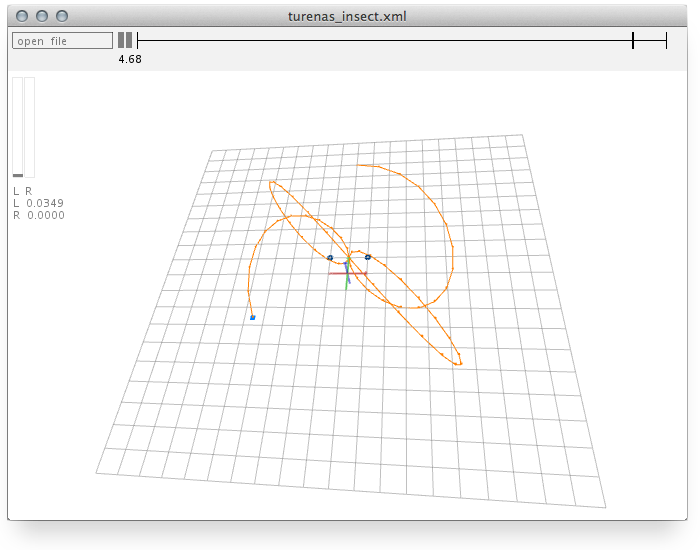
\includegraphics[width=\columnwidth]{of_screenshot.png}
	\caption{OpenFrameworks implementation of SpatDIF, demonstrating again the playback of the `insect' trajectory from `Turenas'} 
	\label{fig:screenshot3}
\end{figure}

\section{Conclusions and Future work}\label{sec:conclusions_future_work}

% COMMENT: Do we want to discuss issues with the specification that the implementation has brought up (such as describing time using floats in 32-bit applications)?

In this article we have shown concrete implementations of the Spatial Sound Description Interchange Format in software.
The examples presented here show limited use-cases, which need to be worked out more fully in a real-life applications.
The intention is to provide a simple method for working with SpatDIF in audio coding environments that is flexible enough to handle all layers of a spatial audio workflow \cite{PetersSMC09}.
A greater challenge is the application of these tools in commercial hosts, in particular DAWs that only expose a small part of their structure, for example to the access by plug-ins.

A short-term goal of this project is the complete implementation of the SpatDIF specification version 0.3 \cite{SpatDIF_03} within the C++ library.
In addition, the methods for purely OSC-driven input and output have to be completed as well as loading and saving of scenes in other markup languages such as JSON.

% TODO
% A short-term goal is the complete implementation of the existing specification within the library.
% A long-term perspective is to develop additional extensions that will further increase the utility of the SpatDIF format.

In a wider perspective, the definitions of further extensions, as laid out in the current specification, will increase the utility of SpatDIF.
In addition, the introduction of new entities, for example of `room' type should enable the description of room acoustics in the reverb extension.
The next round of specification will build on the experience gathered while implementing SpatDIF in the code shown here and will take less effort to integrate into the library, external and addons thanks to its consistent and open design.

%The limited space of this article prevents us from providing full code examples, but 
The external, its source code and the C++ implementation are open-source and may be obtained via git from:\\ \footnotesize\url{http://code.zhdk.ch/git/spatdifrenderer.git}.\normalsize

% \vspace{0.5cm}

\begin{acknowledgments}
This development is funded by the Institute for Computer Music and Sound Technology of the Zurich University of the Arts.
\end{acknowledgments} 

\printbibliography

\end{document}
